\chapter{ANGULAR SENSING AND CONTROL SUPPORTING MATERIAL}



\section{Optical Lever Open Loop Transfer Function}
\label{sec:oplevOLG}
The optical lever open loop transfer function for ETMX is shown in
Fig.~\ref{fig:oplevOLG}. The measurement was made when the
interferometer was unlocked and only the optical lever and OSEM
damping loops on. Because of the two unity gain crossings, one at
2.2~Hz and one at 0.2~Hz, the optical lever loop provides only AC
(velocity) damping. There is no DC control. 

The model uses the pendulum torque to angle transfer function as the
plant and the filters used during Enhanced LIGO as the control. I use
the meausurement to tune the pedulum parameters in the model to best
determine the actual damping coefficient and resonant frequency. For
ETMX, we find the pitch resonant frequency to be 0.65~Hz, 8\%
different from the theoretical 0.6~Hz. Also, we measure the ETMX
damping coefficient to be 0.02.

% Make table of parameters determined for each optic for which I have a measurement?

\begin{figure}
\begin{centering}
\subfigure{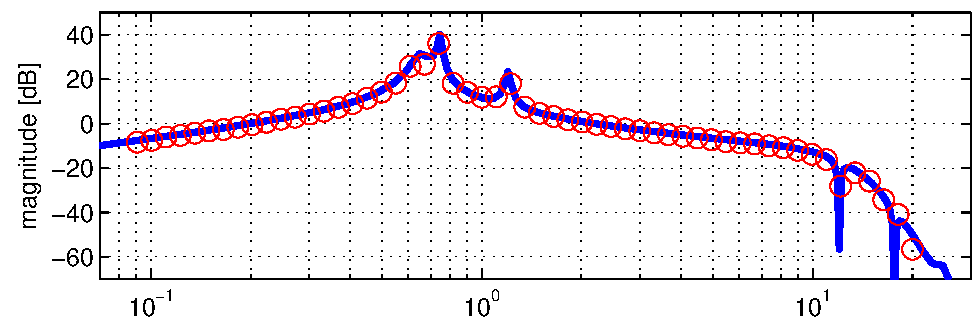
\includegraphics[width=1.0\textwidth]{figures/oplevEX_mags.pdf}}
\subfigure{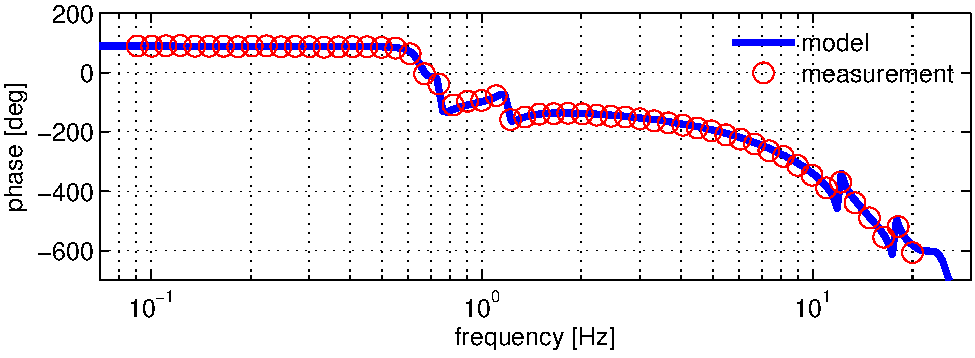
\includegraphics[width=1.0\textwidth]{figures/oplevEX_phases.pdf}}
\caption[Optical lever open loop transfer function]{ETMX pitch optical
  lever open loop transfer function. The model of the plant is tuned
  to match the data, resulting in a pitch resonance of 0.65 Hz and a
  damping factor of $\gamma$ = 0.02. The UGF is at 2.2~Hz and the
  phase margin is $38^\circ$.}
\label{fig:oplevOLG}
\end{centering}
\end{figure}





\section{Misaligned Cavity Axis}
\label{sec:misaligned_cavity}
Here I provide the geometric argument that shows how to calculate the
tilt $a$ and displacement $\alpha$ of a cavity as a function of mirror
misalignment. Cavity tilt is defined by the angle formed between
the line that connects the two beam spots (as given by Eq. \ref{eq:x}) and the line joining the
centers of the mirrors. Cavity displacement uses the same two lines,
yet is defined by the distance between them at the location of the
waist of the resonant spatial mode. Based on pure geometry, the cavity
displacement and tilt are:
\begin{equation}
\left\llbracket \begin{array}{c}
a \\
\alpha \end{array} \right\rrbracket = \frac{1}{L}
\left\llbracket \begin{array}{cc}
z_2 & z_1\\
-1 & 1\end{array} \right\rrbracket
\left\llbracket \begin{array}{c}
x_1\\
x_2 \end{array} \right\rrbracket
\label{eq:cavitydisptilt}
\end{equation}
where $z_i$ is the distance to the waist from mirror $i$ calculated as:
\begin{eqnarray}
z_1 &=& \frac{g_2 (1-g_1) L}{g_1+g_2 - 2 g_1g_2} \\
z_2 &=& L - z_1.
\end{eqnarray}

Clearly, we can combine Eqs. (\ref{eq:x}) and
(\ref{eq:cavitydisptilt}) to arrive at an equation directly relating
mirror tilt to cavity displacement and tilt: 
\begin{equation}
\left\llbracket \begin{array}{c}
a \\
\alpha \end{array} \right\rrbracket = \frac{1}{1-g_1g_2}
\left\llbracket \begin{array}{cc}
g_2z_2 + z_1 & z_2 + g_1z_1\\
-g_2 + 1 & -1 + g_1\end{array} \right\rrbracket
\left\llbracket \begin{array}{c}
\theta_1\\
\theta_2 \end{array} \right\rrbracket.
\label{eq:cavitydisptilt_mirrorangle}
\end{equation}



\section{Power in a Misaligned Cavity}
\label{sec:cavitypower}
I'll show how to calculate the power in a cavity as a function of
cavity axis displacement and tilt. Combined with the results of
Eq. \ref{eq:cavitydisptilt_mirrorangle} we determine how the power
build-up in a cavity depends on a single mirror's angular
displacement.
% %This can be compared with data to calibrate
% %the optical lever error signals as will be shown in Section \ref{sec:oplevcal}. 

The field of a lowest-order Gaussian laser beam along one axis at the beam waist is:
\begin{equation}
\psi(x) = U_0(x) = \left[ \frac{2}{\pi w_0^2} \right]^{1/4} \exp{\left[-\left[\frac{x}{w_0}\right]^2\right]}
\end{equation}
where $w_0$ is the beam waist radius and $U_0$ is the lowest-order
Hermite polynomial. The Hermite polynomials are orthonormal,
ie. $\langle U_i \mid U_j \rangle = \delta_{ij}$. For example, the
next to lowest order polynomial is:
\begin{equation}
U_1(x) = \left( \frac{2}{\pi w_0^2} \right)^{1/4} \frac{2x}{w_0}
\exp{[-(x/w_0)^2]} = \frac{2x}{w_0} U_0(x)
\end{equation}

\subsection{Displaced Cavity}
The field of a cavity with a \emph{displaced} z-axis at the cavity waist is:
\begin{align}
\psi \prime (x) =& \psi(x-a) \\
 =& U_0(x-a) \\
 =& c_0U_0(x) + c_1 U_1(x) + c_2 U_2(x) + ...\\
\end{align}
where $a$ is the displacement of the axis and $c_i$ are constants.

%\subsubsection{Power} 
We want to know $c_0$, the projection of the displaced cavity field onto the beam field: 
\begin{eqnarray}
c_0 &=& \langle \psi \mid \psi \prime \rangle \\
&=& \int_{-\infty}^\infty \psi(x) \psi \prime(x) \, dx \\
 &=& \exp{[-a^2/2 w_0^2]}
\label{eq:c_0}
\end{eqnarray}
The power in this mode is the square of the overlap of the two fields: 
\begin{eqnarray}
P_0&=& \left| \langle \psi \mid \psi \prime \rangle \right| ^2\\ 
&=& \exp{[-[a/w_0]^2]} 
\end{eqnarray}

%\subsubsection{$U_1$ field}
For the purpose of wavefront sensing, we need to know the amplitude,
$c_1$, of the first order $U_1$ field. This can be approximated as
demonstrated in Anderson \cite{Anderson1984Alignment} using
the Taylor series expansion of the exponential in $\psi \prime(x) =
U_0(x-a)$, assuming a displacement $a$ that's small compared to waist
size $w_0$.
\begin{eqnarray}
\psi \prime(x) &=& \left[ \frac{2}{\pi w_0^2} \right]^{1/4}
\exp{\left[-\left[\frac{x-a}{w_0}\right]^2\right]} \\
&=& \left[ \frac{2}{\pi w_0^2} \right]^{1/4} \left[1 -
  \left[\frac{x-a}{w_0} \right]^2 + \mathcal{O}(a^4) \right] \\
&=& \left[ \frac{2}{\pi w_0^2} \right]^{1/4} \left[ \frac{2xa}{w_0^2}
  \left[1-\frac{x^2}{w_0^2} + ... \right] + \left[ 1 -
    \frac{x^2}{w_0^2} + \frac{1}{2} \frac{x^4}{w_0^4}
    - ... \right] + \mathcal{O}(a^2) \right] \\
&=& \left[ \frac{2}{\pi w_0^2} \right]^{1/4} \left[1 +
  \frac{2xa}{w_0^2} + \mathcal{O}(a^2) \right] \exp{\left[ -\left[\frac{x}{w_0}\right]^2
  \right]} \\
&=& U_0(x) + \frac{a}{w_0} U_1(x) + ...
\end{eqnarray}
Notice that here we find $c_0 = 1$, which is consistent with the
exact result of Eq.~\ref{eq:c_0} when we apply our $a^2 \approx 0$
approximation. We find that the amplitude of the first order
Hermite-Gauss field for a displaced cavity is
\begin{equation}c_1 = a/w_0.
\end{equation}



\subsection{Tilted Cavity}
The field of a cavity with a \emph{tilted} z-axis at the cavity waist is a tad more complex to derive. We assume the tilt, $\alpha$, is small such that $\sin{\alpha} \approx \alpha$ and $\cos{\alpha} \approx 1$. Also, we assume the beam divergence angle, $\theta_0=\lambda / \pi w_0$, is small such that the wavefronts near the waist can be considered parallel to one another. 

Here, the important quantity to consider is the phase of the cavity field at the cross-section of the beam waist.  The phase is either advanced or retarded compared to that of the beam:
\begin{eqnarray}
\psi \prime(x) &=& \psi(x \prime) \exp{[-i k z \prime]} \\
 & \approx& \psi(x \cos{\alpha}) \exp{[-i k x \sin{\alpha}]} \\
 &\approx& \psi(x) \exp{[- i k x \alpha]} \\
 &=& U_0(x) \exp{[- i k x \alpha]}
\label{eq:psi_tilted}
\end{eqnarray}
where $k=2\pi / \lambda$ and $\lambda$ is the wavelength of the laser light.

%\subsubsection{Power} 
The overlap of the fields of the beam and tilted cavity is $ \exp{[-\alpha^2/2 \theta_0^2]} $. Therefore the power is:
\begin{equation}
P_0 = \exp{[-(\alpha/\theta_0)^2]}.
\end{equation}

%\subsubsection{$U_1$ field}
An expansion of the exponential in Eq. \ref{eq:psi_tilted} for a small
tilt $\alpha$ gives:
\begin{eqnarray}
\psi \prime(x) &=& U_0(x) [1 + i k x \alpha + \mathcal{O}(\alpha^2) ] \\
&=& U_0(x) + \frac{i k \alpha w_0}{2} U_1(x) + \mathcal{O}(\alpha^2).
\end{eqnarray}
Therefore, the amplitude of the first order Hermite-Gauss field for a
tilted cavity is 
\begin{equation}
c_1 = i k \alpha w_0 / 2.
\end{equation}


\subsection{Displaced and Tilted Cavity}
The most general case, of course, is to have a cavity axis that is both displaced \emph{and} tilted at the beam waist:
\begin{equation}
\psi \prime(x) = \psi(x-a) \exp{[-i k (x-a) \alpha]}.
\end{equation}
We find:
\begin{equation}
\langle \psi \mid \psi \prime \rangle = \exp{\left[- \frac{a^2}{2 w_0^2} \right]} \exp{\left[-\frac{\alpha^2}{2 \theta_0^2}\right]} \exp{\left[- \frac{i a \alpha}{x_0 \theta_0}\right]}
\end{equation}
and
\begin{equation}
P_0 = \exp{\left[- \frac{a^2}{w_0^2} \right]}
\exp{\left[-\frac{\alpha^2}{\theta_0^2}\right]}.
\label{eq:pwr_disptilt}
\end{equation}



\section{Initial DC Alignment of the Interferometer}
\label{sec:initial_alignment}
After any kind of in-vacuum work, the DC alignment of the mirrors is
usually too poor for the interferometer to lock. A bootstrapping
process of tweaking the alignment by hand is necessary, assuming the
mirrors start out pointing in generally the right direction, as is
usually the case. As pointed out in Sec.~\ref{sec:alignment_overview}, the
QPDs at the end stations are the fixed reference points for the
overall alignment, so this process begins with making sure the light
reaches them. We then adjust the rest of the mirrors to maximize power
build-up in the arms and to maximze spatial overlap of the light
reflected from each arm.

An outline of the process is presented here. ``Misalign'' means to
intentionally point a mirror so far away from any known good positions
as to eliminate it from the configuration.  ``Align'' and ``restore''
mean to bring a mirror or configuration to the best known
position(s). Centering the beam on a mirror is accomplished by using
the suspension cage surrounding the mirror as a reference. Camera
images and QPD readback provide the signals used for beam centering. 

\begin{itemize}
\item[] \textbf{X-arm} \vspace{-10pt}
\item restore the x-arm (misalign RM, ITMY, and ETMY, align ITMX and ETMX) \vspace{-10pt}
\item use ITMX to center the beam on QPDX \vspace{-10pt}
\item use ETMX to center the beam on ITMX \vspace{-10pt}
\item with x-arm locked, use MMT3 to maximize the x-arm power build-up (NPTRX, can expect
  about 95\%) \vspace{-10pt}
\item save the MMT3, ITMX, and ETMX alignment settings 
\item[] \textbf{Y-arm} \vspace{-10pt}
\item restore the y-arm (misalign ITMX and ETMX, align ITMY and ETMY) \vspace{-10pt}
\item use ITMY to center the beam on QPDY \vspace{-10pt}
\item use ETMY to center the beam on ITMY \vspace{-10pt}
\item with y-arm locked, use BS to maximize the y-arm power build-up (NPTRY, can expect
  about 90\%) \vspace{-10pt}
\item save the BS, ITMY, and ETMY alignment settings 
\item[] \textbf{Relative x-arm and y-arm} \vspace{-10pt}
\item note AS beam position on camera while toggling between x-arm and
  y-arm locks\vspace{-10pt}
\item use ETMs to align the two AS beams \vspace{-10pt}
\item restore the Michelson (misalign ETMs, align ITMs) \vspace{-10pt}
\item use BS to make AS port as dark as possible \vspace{-10pt}
\item re-do y-arm alignment if ambitious 
\item[] \textbf{Recycling mirror} \vspace{-10pt}
\item restore the PRM (misalign ETMs, align ITMs and RM)
  \vspace{-10pt}
\item use RM to center beam on ETMY cage 
\item[] \textbf{Restore full interferometer--off you go!}
\end{itemize}






% \section{Seismic Contributions to Optical Lever Spectra}
% \label{sec:oplev_contributions}
% Wiener filtering \cite{Wiener1975Extrapolation} is a useful method to
% determine the likeness of two signals. In short, the Wiener filter
% coefficients are chosen to minimize the mean square difference between
% a Wiener filtered signal and a reference time series. If one signal is
% derived from the other, then there exists a Wiener filter that can
% precisely transform one signal into the other.



% The optical lever error signals ideally witness the mirror motion,
% which in turn is expected to come from the ground's motions. The
% optical lever signal, may, however, be contaminated by optical lever
% sensing (electronics) noise or acoustic couplings. It is therefore
% informative to calculate Wiener filters for the sesimometer signals to
% understand how much of the optical lever spectra are in fact due to
% ground motion. The contributions of the three seismometers to each
% large optic optical lever are shown in
% Fig.~\ref{fig:OLcontributions}. We see that the optical lever signals
% are almost entirely explained by ground motion, with the notable
% exceptions being a peak between 3 and 4~Hz for ITMY, and 0.3 and
% 0.7~Hz for the RM, and broadband extra motion for the BS.

% Furthermore, the relative magnitudes of the contributions from the
% three seismometers make sense. Greater than 1~Hz, coherence is
% greatest with the nearest seismometer, and less than 1~Hz,
% seismometers contribute more equally (except for the ITMs, which are
% everywhere very coherent with the corner station seismometer).

% \begin{figure}
% \begin{centering}
% \subfigure{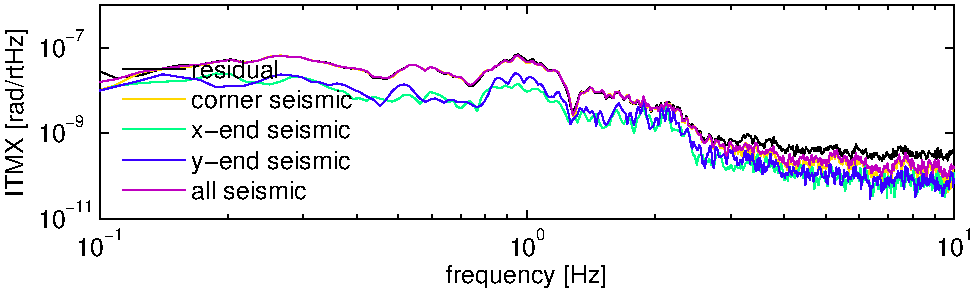
\includegraphics[width=1.0\textwidth]{figures/nolockIX.pdf}}
% \subfigure{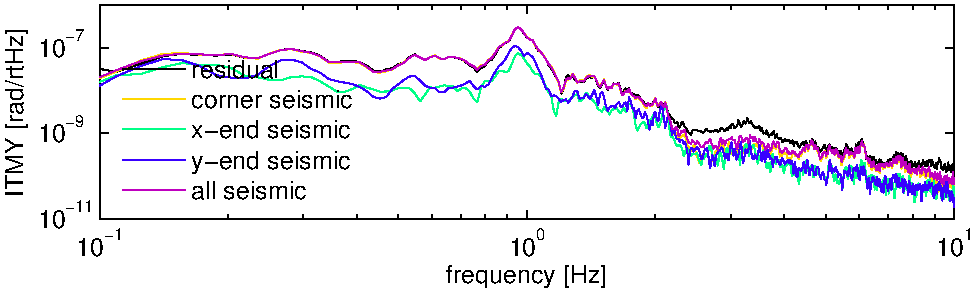
\includegraphics[width=1.0\textwidth]{figures/nolockIY.pdf}}
% \subfigure{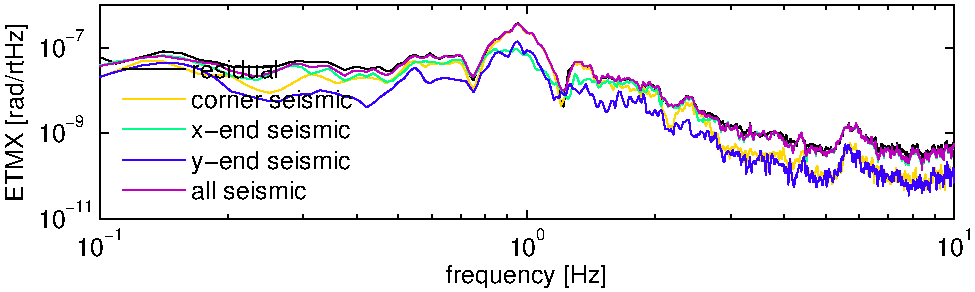
\includegraphics[width=1.0\textwidth]{figures/nolockEX.pdf}}
% \subfigure{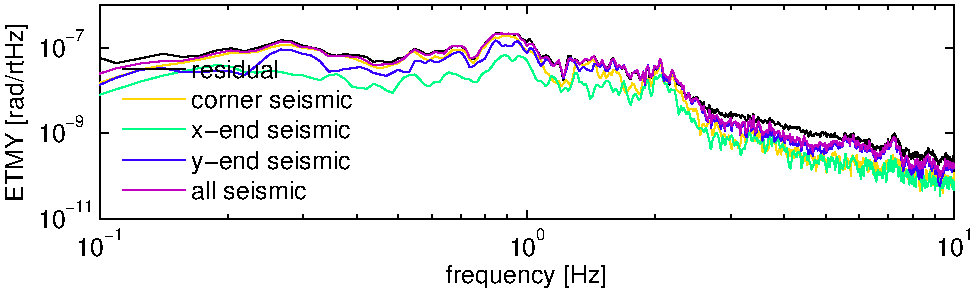
\includegraphics[width=1.0\textwidth]{figures/nolockEY.pdf}}
% \caption[Contribution of sesimic noise to optical lever error
% signal]{Contribution of sesimic noise to optical lever error signal
%   (called residual). The interferometer was unlocked and optical lever
%   and OSEM AC damping present.}
% \label{fig:OLcontributions}
% \end{centering}
% \end{figure}

% \begin{figure}
% \begin{centering}
% \subfigure{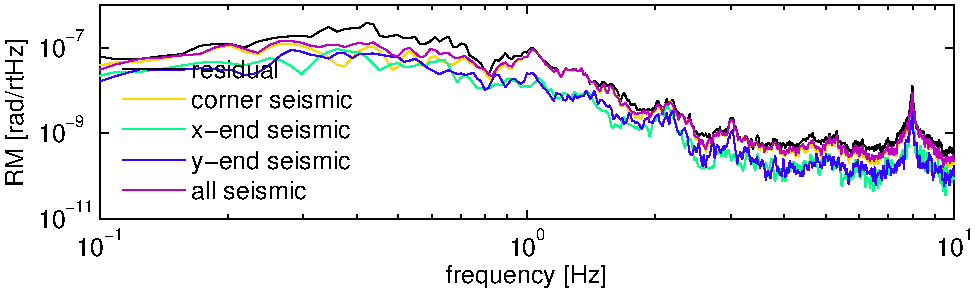
\includegraphics[width=1.0\textwidth]{figures/nolockRM.pdf}}
% \subfigure{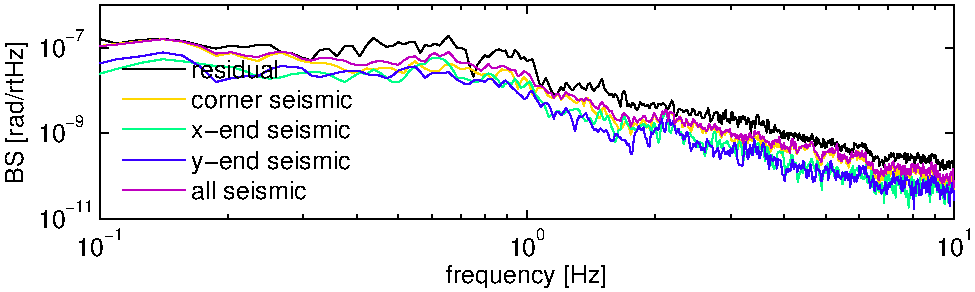
\includegraphics[width=1.0\textwidth]{figures/nolockBS.pdf}}
% \subfigure{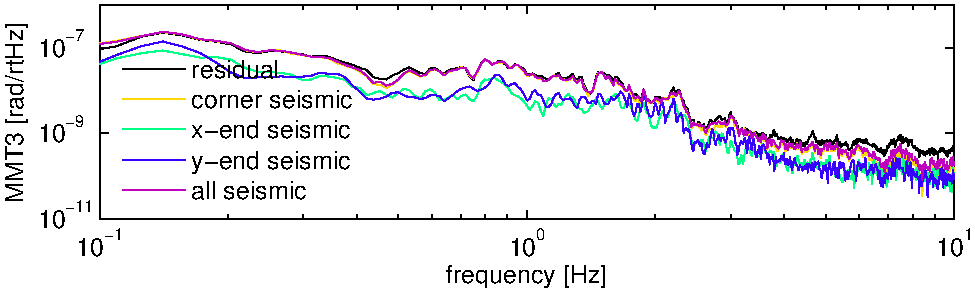
\includegraphics[width=1.0\textwidth]{figures/nolockMMT3.pdf}}
% %\caption[]{Fig.~\ref{fig:OLcontributions} continued.}
% Fig.~\ref{fig:OLcontributions} continued.
% \end{centering}
% \end{figure}



% \section{Photodiodes}
% \label{sec:pds}
% The basic photoconductive photodiode is depicted in Fig. \ref{}. A
% negative voltage applied to the anode, represented by the line, does
% not yield any current across the photodiode until electrons are
% released by the energy of photons striking the diode. Electrons flow
% in the direction of the cathode which is connected to ground,
% producing a current
% \begin{equation}
% i_\gamma = \frac{q_e}{h \nu} P \epsilon
% \end{equation}
% where $q_e$ is the electron charge, $h$ is Planck's constant, $\nu$ is
% the frequency of the incident light, $P$ is the power of the light,
% and $\epsilon$ is the quantum efficiency of the diode. The quantity
% $q_e/h \nu$ is known as the \emph{responsivity}. For LIGO where
% $\lambda = 1064$ nm, the responsivity is $0.86$ A/W.



% \section{Channel Names}
% \textcolor{blue}{finish this or skip!}
% It is often perplexing why there are so many channels with almost
% identical names. And just what those names mean can also sometimes be
% elusive. The best advice I have to offer about how to figure out for
% one's self what the root of the channel name conveys about the data it
% represents is to browse the MEDM screens. The MEDM screens pictorially
% show the flow of which channels are derived from others, and whether
% they sit before or after an excitation point, for example. They also
% sometimes offer hints as to exactly what calculation is done under the
% scene in the front-end code to compute new channels. 

% The topic I want to cover here is the difference between the
% \texttt{OUT}, \texttt{OUT16}, \texttt{OUTPUT}, and \texttt{OUTMON}
% channel name extenstions. They appear in all of the subsystems, and it
% is crucial to realize that some are good for analyzing data and some
% good for getting only a sense in real-time of what's going on. Some
% are typically recorded to disk, and some are not. These concepts
% extend to other common name extensions as well. 




\section{Parameters}
Table \ref{tab:ROCs} shows the radii of curvature (ROC) of the Enhanced LIGO mirrors. 
\begin{table}
\centering
\caption{Mirror radii of curvatures.} 
%References are \cite{Adhikari2005Input} and \href{http://www.ligo.caltech.edu/~gari/COCAsBuilt.htm}{Garilynn Billingsley's website}
\begin{tabular}{l r@{}l r@{}l}
\hline
optic & \multicolumn{2}{l}{L1 ROC [km]} & \multicolumn{2}{l}{H1 ROC [km]} \\
\hline
MC1 & 0&.01725 & & \\
MC2 & 80&  & & \\ 
MC3 & 0&.01725 & & \\ 
MMT1 & 6&.76 & 6&.77 \\
MMT2 & 3&.16 & 3&.17 \\
MMT3 & 25&.16 & 25&.04\\
RM & 15&.78 & 14&.40 \\
BS & -189& & -336& \\
ITMX & 14&.760 & 13&.910 \\ 
ITMY & 14&.520 & 13&.600 \\
ETMX & 8&.730 & 7&.260 \\
ETMY & 8&.720 & 7&.320 \\
\hline
\end{tabular}
\label{tab:ROCs}
\end{table} 




\section{Seismic Spectra}
\label{sec:groundmotion}
There are three seismometers at LLO for the purpose of monitoring the
ground motion at the corner station (LVEA) and two end stations. The
calibration for the digitally collected data is $2.4 \times 10^{-9}$
m/s/count. As stated in the introduction of
Ch.~\ref{ch:characterization}, I include here snapshots of the ground
motion at the time of ground motion-sensitive measurements. Each
spectra represents 30~minutes of data centered around the time of the
measurement. There are three degrees of freedom for each seismometer,
$x$, $y$, and $z$. They are aligned with the interferometer's $x$ and
$y$ arm coordinate system.

Although the interferometer is very sensitive to ground motion, the
range of seismic activity for which it can maintain full lock is
reasonably large. The microseism (0.1-0.35~Hz) varies by factors of
several seasonally (it's worse in the winter), and the 1-3~Hz motion
varies by factors of several from day to night. Seismic motion the
interferometer typically cannot handle includes events like
earthquakes (0.03-0.1~Hz) and heavy activity on site (3-10~Hz). Motion
at these frequencies are otherwise constant and at a level so as to
not affect interferometer operation. 

\begin{figure}
\begin{centering}
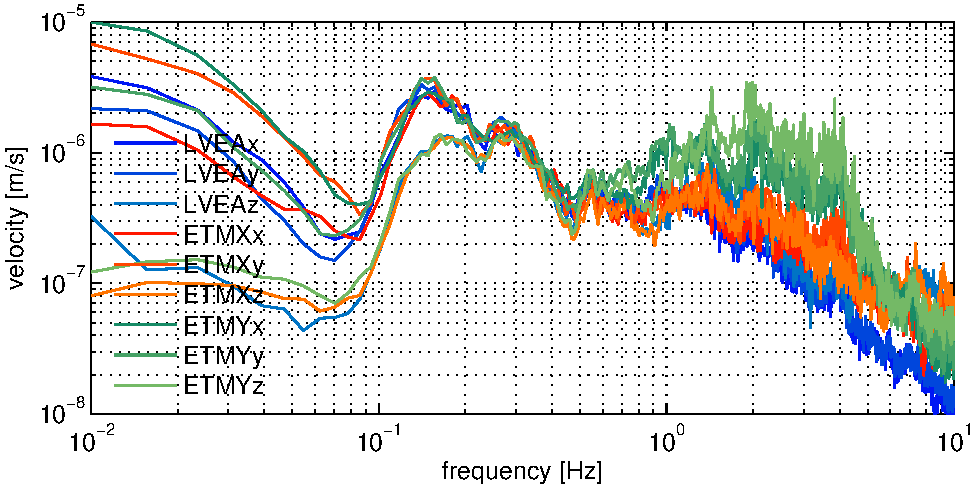
\includegraphics[width=1.0\textwidth]{figures/seis956751915_nolock.pdf}
\caption[]{Ground motion at time of optical lever spectra when the
  interferometer was unlocked (Fig.~\ref{fig:seismicMirror}) and at
  time of ASC suppression demonstration (Fig.~\ref{fig:ASConoff}). GPS
  time is 956751915 (May 1, 2010 07:25 CDT).}
\label{fig:seismic_nolock}
\end{centering}
\end{figure}

\begin{figure}
\begin{centering}
\includegraphics[width=1.0\textwidth]{figures/seis956754915.pdf}
\caption[]{Ground motion at time of ASC suppression demonstration
  (Fig.~\ref{fig:ASConoff}). GPS time is 956751915 (May 1, 2010 08:15
  CDT).}
\label{fig:seismic_locked}
\end{centering}
\end{figure}

\begin{figure}
\begin{centering}
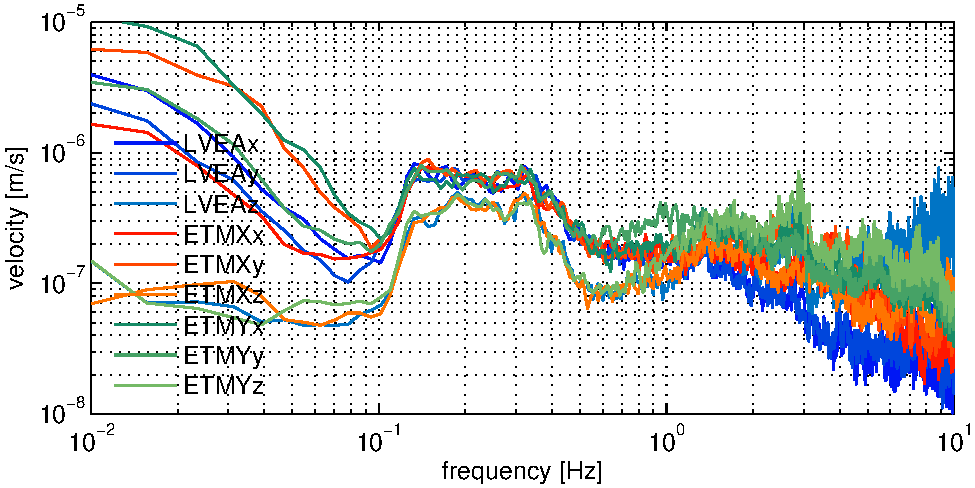
\includegraphics[width=1.0\textwidth]{figures/seis971128215_highWFSgain.pdf}
\caption[]{Ground motion at time of input beam motion impression
  measurement (Fig.~\ref{fig:inputbeam_impression}). GPS time is
  971128215 (Oct. 14, 2010 16:50 CDT).}
\label{fig:seismic_highgain}
\end{centering}
\end{figure}

\begin{figure}
\begin{centering}
\includegraphics[width=1.0\textwidth]{figures/seis956728935.pdf}
\caption[]{Ground motion at time of beam spot motion measurement
  (Fig.~\ref{fig:bsm}). GPS time is 956728935 (May 1, 2010 01:02
  CDT).}
\label{fig:seismic_bsm}
\end{centering}
\end{figure}


\begin{figure}
\begin{centering}
\includegraphics[width=1.0\textwidth]{figures/seis958456964.pdf}
\caption[]{Ground motion at time of ASC to DARM noisebudget plot
  (Fig.~\ref{fig:asc2darm}). GPS time is 958456964 (May 21, 2010 01:02
  CDT).}
\label{fig:seismic_NB}
\end{centering}
\end{figure}




